\documentclass[11pt]{article}

\usepackage{preprint}
\usepackage{amsmath, amsthm, amssymb, amsfonts}
\usepackage{resizegather}
\usepackage[numbers,square]{natbib}
\usepackage[utf8]{inputenc}
\usepackage[T1]{fontenc}
\usepackage{xcolor}
\usepackage[colorlinks = true,
    linkcolor = purple,
    urlcolor  = blue,
    citecolor = cyan,
    anchorcolor = black]{hyperref}
\usepackage{booktabs}
\usepackage{multirow}
\usepackage{nicefrac}
\usepackage{microtype}
\usepackage{lineno}
\usepackage{float}
\usepackage[shortlabels]{enumitem}
\usepackage{float}
\usepackage{subfloat}
\usepackage{caption}
\usepackage{subcaption}
\usepackage{amssymb}
\usepackage{bbold}
\usepackage{stmaryrd}
\usepackage{graphicx}
\usepackage{hyperref}
\usepackage{titlesec}
\usepackage{authblk}
\usepackage{graphics}
\usepackage[font=small,labelfont=bf]{caption}
\usepackage{algorithm}
\usepackage[noend]{algpseudocode}
\captionsetup[subfigure]{justification=centering}

\setlength{\belowcaptionskip}{-10pt}
\newcommand{\specialcell}[2][c]{%
  \begin{tabular}[#1]{@{}c@{}}#2\end{tabular}}


\bibliographystyle{unsrtnat}
\setlist[enumerate,1]{leftmargin=2em}
\titlespacing\section{0pt}{0.1ex plus 0.2ex minus 0.1ex}{0.1ex plus 0.2ex minus 0.1ex}
\titlespacing\subsection{0pt}{0.1ex plus 0.2ex minus 0.1ex}{0.1ex plus 0.2ex minus 0.1ex}

\renewcommand*{\Authfont}{\bfseries}

\newcommand{\R}{\mathbb{R}}
\newcommand{\N}{\mathbb{N}}
\DeclareMathOperator*{\argmin}{arg\,min}
\DeclareMathOperator*{\argmax}{arg\,max}
\DeclareMathOperator*{\minimize}{minimize}
\DeclareMathOperator*{\Argmin}{\text{Argmin}}
\DeclareMathOperator*{\Argmax}{\text{Argmax}}
\DeclareMathOperator*{\Cost}{\text{Cost}}

\title{Generative modeling project : Neural Optimal Transport}
\author[1]{Paul Barbier}
\author[1]{Bastien Le Chenadec}
\affil[1]{École des Ponts ParisTech, Master MVA}

\begin{document}

\maketitle

\section{Introduction}

Optimal Transport (OT) is a mathematical framework that aims to find the most efficient way to transport a distribution of mass to another. This framework has been used extensively in the context of generative models, for instance as a loss function in the training of Generative Adversarial Networks (GANs) or by learning a mapping between two distributions. In this project, we aim to study the paper "Neural Optimal Transport" (Korotin, 2023) \cite{korotin-2022} which introduces an algorithm to train a neural network to learn the optimal transport between two distributions, with applications in image generation. We will introduce some optimal transport problems in various formulations, but we will focus on giving a general overview and some details and hypotheses will be omitted for the sake of clarity.

\section{Background on Optimal Transport}

\subsection{Optimal Transport Problem}

Let $\mu$ and $\nu$ be two probability distributions on $\mathcal{X}$ and $\mathcal{Y}$ respectively (typically $\mathcal{X}, \mathcal{Y}=\R^n,\R^m$). To give a meaning to "efficiently" transporting mass, we define a cost function $c:\mathcal{X}\times\mathcal{Y}\to\R$ that quantifies the cost of transporting a unit of mass in $\mathcal{X}$ to one in $\mathcal{Y}$. The (Monge) optimal transport problem consists in finding a \textbf{transport map} $T^*:\mathcal{X}\to \mathcal{Y}$ such that :
\begin{equation}
    T^* \in \Argmin_{T\#\mu=\nu} \int_{\mathcal{X}} c(x,T(x))d\mu(x) \quad\quad \Cost(\mu,\nu) = \int_{\mathcal{X}} c(x,T^*(x))d\mu(x)
\end{equation}
where $T\#\mu$ is the pushforward distribution of $\mu$ by $T$, defined by $(T\#\mu)(A)=\mu(T^{-1}(A))$ for any measurable set $A\subset\mathcal{Y}$. This formulation calls for a deterministic mapping from $\mathcal{X}$ to $\mathcal{Y}$, which is not always desirable or feasible under general assumptions. Kantorovich introduced  a relaxed OT problem that aims at finding a \textbf{transport plan} $\pi^*\in \Pi(\mu,\nu)$ in the set of joint distributions on $\mathcal{X}\times\mathcal{Y}$ with marginals $\mu$ and $\nu$ such that :
\begin{equation}
    \pi^* \in \Argmin_{\pi\in\Pi(\mu,\nu)} \int_{\mathcal{X}\times\mathcal{Y}} c(x,y)d\pi(x,y) \quad\quad \Cost(\mu,\nu) = \int_{\mathcal{X}\times\mathcal{Y}} c(x,y)d\pi^*(x,y)
\end{equation}
In general the solution to the Kantorovich problem is stochastic, but in some cases it may be deterministic in which case it is also a solution to the Monge problem. Building on this idea of stochasticity in the solution, weak OT was introduced as a generalization of the Kantorovich problem, where the cost function is of the form $C: \mathcal{X}\times \mathcal{P}(\mathcal{Y})\to\R$. In this case the weak OT problem writes :
\begin{equation}
    \pi^* \in \Argmin_{\pi\in\Pi(\mu,\nu)} \int_{\mathcal{X}} C(x,\pi(\cdot|x))d\pi(x) \quad\quad \Cost(\mu,\nu) = \int_{\mathcal{X}} C(x,\pi^*(\cdot|x))d\pi^*(x)
\end{equation}
where $\pi(\cdot|x)$ is the conditional distribution of $\pi$ given $x$ and $d\pi(x)$ is the marginal distribution of $\pi$ on $\mathcal{X}$ (which is actually $\mu$).

\subsection{Weak OT duality}

For weak OT cost $C$, and $f$ defined on $\mathcal{Y}$ sufficiently regular, the weak C-transform of $f$ is defined on $\mathcal{X}$ as :
\begin{equation}
    f^C(x) = \inf_{\rho\in \mathcal{P}(\mathcal{Y})} \left\{C(x,\rho)-\int_{\mathcal{Y}}f(y)d\rho(y)\right\}
\end{equation}
The dual form of the weak OT problem is then :
\begin{equation}
    f^*\in\Argmax_{f} \int_{\mathcal{X}} f^C(x)d\mu(x) + \int_{\mathcal{Y}} f(y)d\nu(y) \quad\quad \Cost(\mu,\nu) = \int_{\mathcal{X}} f^{*C}(x)d\mu(x) + \int_{\mathcal{Y}} f^*(y)d\nu(y)
\end{equation}

\section{Neural Optimal Transport}

In (Korotin, 2023) \cite{korotin-2022}, the authors aim to solve the weak OT problem with a neural network. First they reformulate the weak dual problem with noise outsourcing, then they introduce an algorithm to solve this problem.

\subsection{Weak dual OT reformulation}

From now on we consider $\mathcal{X}\subset\R^n$ and $\mathcal{Y}\subset\R^m$. We introduce $\mathcal{Z}\subset\R^d$ a latent space with a distribution $\rho\in \mathcal{P}(\mathcal{Z})$. The following result holds true under some basic assumptions on $\rho$ :
\begin{equation}
    f^C(x)=\inf_t \left\{C(x, T\#\rho)-\int_{\mathcal{Z}}f(t(z))d\rho(z)\right\}
\end{equation}
This result can be integrated against $\mu$ to replace the dual weak OT problem by a maximin problem :
\begin{align}
    \begin{split}
        \Cost(\mu,\nu) & = \sup_{f} \inf_{T}
        \int_{\mathcal{Y}}f(y)d\nu(y) + \int_{\mathcal{X}} \left( C(x, T(x,\cdot)\#\rho)-\int_{\mathcal{Z}}f(T(x,z))d\rho(z)\right)d\mu(x) \\
                       & = \sup_{f} \inf_{T} \mathcal{L}(f,T)
    \end{split}
    \label{eq:weak_ot_reformulation}
\end{align}
where $T:\mathcal{X}\times\mathcal{Z}\to\mathcal{Y}$. The proofs of these results are in the paper \cite{korotin-2022}. This reformulation can be interpreted in the following way : the solution to the weak OT problem is a \textbf{stochastic map} $T:\mathcal{X}\times \mathcal{Z}\to \mathcal{Y}$ that is split into two parts, a deterministic part $T(x,\cdot)$ and a stochastic part $z\mapsto T(x,z)$. $\mathcal{Z}$ is a latent space that models the randomness in the transport.

Solving (\ref{eq:weak_ot_reformulation}) does not necessarily yield a solution $T^*$ to the weak OT problem. However under sufficient convexity conditions on $C$ the solution to the maximin problem is a solution to the weak OT problem. With that in mind the authors introduce an algorithm to solve this problem and restrict their attention to such cost functions.

\subsection{SGAD}

The authors prove that the space of neural networks is rich enough to approximate stochastic maps $T$ which motivates the use of neural networks to solve (\ref{eq:weak_ot_reformulation}). $f$ and $T$ in (\ref{eq:weak_ot_reformulation}) are parametrized by neural networks $f_{\omega}$ and $T_{\theta}$ respectively. The authors use a stochastic gradient ascent descent (SGAD) algorithm to solve the problem. The algorithm is presented in Figure \ref{fig:sgad}.

\begin{figure}[H]
    \begin{algorithm}[H]
        \caption{Stochastic Gradient Ascent Descent (SGAD) algorithm for Neural Optimal Transport}
        \begin{algorithmic}[1]
            \State \textbf{Input} : distributions $\mu,\nu,\rho$ accessible by samples, mapping network $T_{\theta}:\mathbb{R}^{m}\times\mathbb{R}^{n}\rightarrow\mathbb{R}^{d}$, potential network $f_{\omega}:\mathbb{R}^{n}\rightarrow\mathbb{R}$, number of inner iterations $K_{T}$, (weak) cost $C:\mathcal{X}\times\mathcal{P}(\mathcal{Y})\rightarrow\mathbb{R}$, empirical estimator $\widehat{C}\big{(}x,T(x,Z)\big{)}$ for the cost
            \State \textbf{Output} : learned stochastic OT map $T_{\theta}$ representing an OT plan between distributions $\mu,\nu$
            \Repeat
            \State Sample batches $Y\sim\nu$, $X\sim\mu$, for each $x\in X$ sample batch $Z_{x}\sim\rho$
            \State $\mathcal{L}_{f}\leftarrow\frac{1}{|X|}\sum_{x\in X}\frac{1}{|Z_{x}|}\sum_{z \in Z_{x}}f_{\omega}\big{(}T_{\theta}(x,z)\big{)}-\frac{1}{|Y|}\sum_{y\in Y}f_{ \omega}(y)$
            \State Update $\omega$ by using $\frac{\partial\mathcal{L}_{f}}{\partial\theta}$
            \For {$k_{T}=1,2,\ldots,K_{T}$}
            \State Sample batch $X\sim\mu$, for each $x\in X$ sample batch $Z_{x}\sim\rho$
            \State $\mathcal{L}_{T}\leftarrow\frac{1}{|X|}\sum_{x\in X}\big{[}\widehat{C}\big{(}x,T_{\theta}(x,Z_{x})\big{)}-\frac{1}{|Z_{x}|}\sum_{z\in Z_{x}}f_{\omega}\big{(} T_{\theta}(x,z)\big{)}\big{]}$
            \State Update $\theta$ by using $\frac{\partial\mathcal{L}_{\theta}}{\partial\theta}$
            \EndFor
            \Until{converged}
        \end{algorithmic}
    \end{algorithm}
    \caption{Neural Optimal Transport algorithm \cite{korotin-2022}}
    \label{fig:sgad}
\end{figure}

\subsection{Application to generative modeling}

Weak optimal transport can be used for generative modeling by learning a stochastic map between two (data) distributions. This stochastic map is learned by a neural network, which is trained to solve the weak optimal transport problem. One appealing aspect of weak optimal transport is that it allows for stochasticity in the solution, which is desirable in many generative modeling tasks such as image generation (for instance generating multiple plausible images from a single input image).

However, learning with weak optimal transport also has its own set of challenges. For instance, the choice of the cost function can be difficult, for instance when the distributions are high-dimensional. Furthermore, the cost function needs to satisfy strict convexity conditions in the context of this paper to ensure that the solution to the maximin problem is a solution to the weak optimal transport problem. The training of the neural network can also be challenging, requiring careful tuning of hyperparameters. It is also subject to the usual challenges of generative modeling, such as mode collapse.

From a theoretical standpoint, weak OT is also challenging because of the non-uniqueness of the solution, and the difficulty to derive theoretical solutions even in simple cases. The authors of the paper consider the weak quadratic cost with $\gamma=1$ for which a unique \textit{class} of solutions exists (i.e. all solutions verify some gradient property), but this is not the case in general.

\section{Experiments}

For this project, we conducted experiments using the code provided by the author. You can find our scripts at \href{https://github.com/bastienlc/NOT}{https://github.com/bastienlc/NOT}. We've done a first experiment with generated synthetic data and a second one with a more realistic use-case using a large dataset.

\subsection{Synthetic data}

First, we conducted experiments using synthetic data on a simple 2D grid. Our spaces $\mathcal{X}$ and $\mathcal{Y}$ are $\R^2$ and we adopt the same $\gamma$-weak quadratic cost function as in the paper (\ref{eq:toy_cost}) (with $\gamma=1$), thus solving the weak OT problem.
\begin{equation}
    C\big{(}x,\mu\big{)}=\int_{\mathcal{Y}}\frac{1}{2}\|x-y\|^{2}d\mu(y)-\frac{1}{2} \text{Var}(\mu)=\frac{1}{2}\|x-\int_{\mathcal{Y}}y\,d\mu(y)\|^{2}
    \label{eq:toy_cost}
\end{equation}
The input distribution is a $2D$ standard normal distribution and the target distribution is a mixture of two semicircles ("moon distribution"). This is not too different from the toy examples in the paper which were either a spiral or a mixture of gaussians.

The networks are simple feedforward neural networks with 2 hidden layers of $100$ hidden units each and ReLU activations. We used similar hyperparameters to the ones in the paper (batch size of $64$, $10$ iterations for the optimization of $T_\theta$, Adam optimizer, $10000$ steps...). The training is straightforward with these parameters, but while experimenting with different ones we found that the model is quite sensitive to the batch size and the number of iterations for the optimization of $T_\theta$.

The main results are shown in Figure~\ref{fig:toy_1}. The results are similar to the ones in the paper with a good mapping of the input distribution to the target distribution. The resulting distribution is a bit more noisy than the target distribution but the general shape is well captured.

In figure \ref{fig:toy_2}, we show the inner workings of the model. The left plot shows the average of the learned transport for different points in the input distribution. On average, points in the center will not move (they will be mapped equally in different directions), while points on the border will be moved towards the center because the input distribution has a bigger support than the target distribution. The middle plot shows the transport for a batch of points; we can see that there is a lot of movement to obtain the target distribution, and also that the same point can sometimes be moved in very different directions. The right plot shows the optimal transport plan obtained with the POT\footnote{https://pythonot.github.io/} library. The learned transport is very close to the optimal transport plan.

\begin{figure}[H]
    \centering
    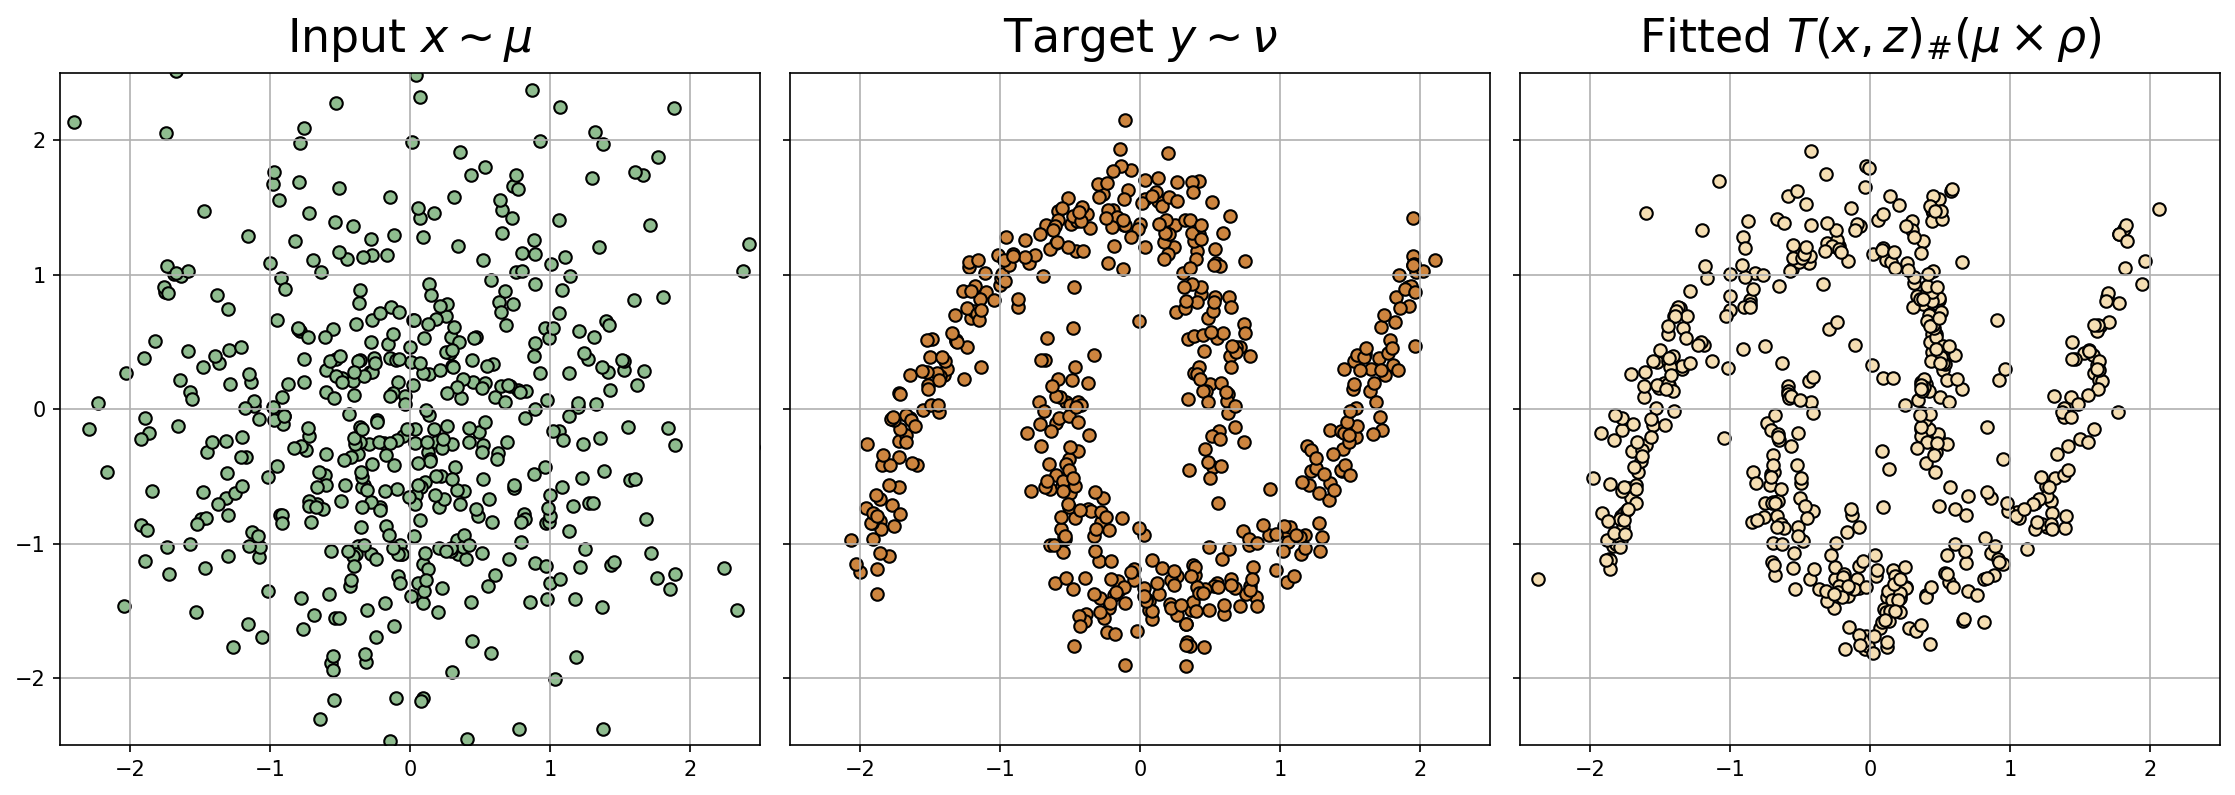
\includegraphics[width=0.9\textwidth]{figures/toy_1.png}
    \caption{Synthetic data experiment. Left: input gaussian distribution. Middle: target distribution. Right: learned transport of the input distribution to the target distribution.}
    \label{fig:toy_1}
\end{figure}

\begin{figure}[H]
    \centering
    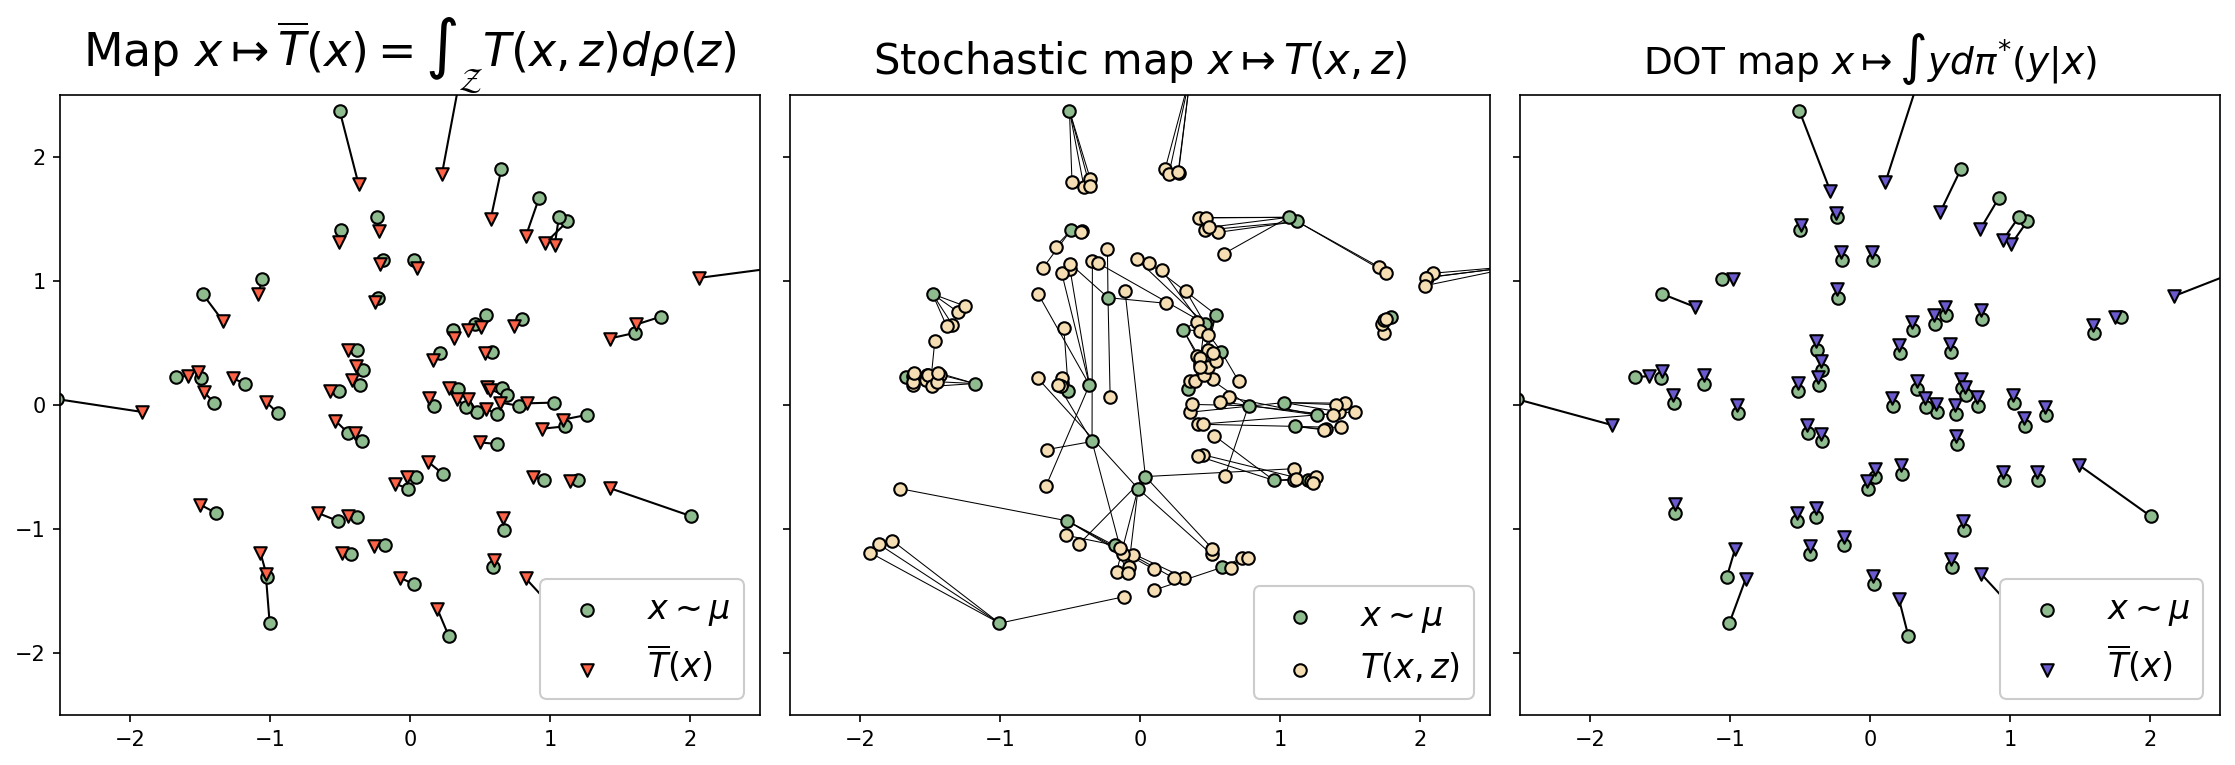
\includegraphics[width=0.9\textwidth]{figures/toy_2.png}
    \caption{Synthetic data experiment. Left: average of the learned transport for different points. Middle: learned transport for a batch of points. Right: optimal transport plan obtained with the POT library.}
    \label{fig:toy_2}
\end{figure}

\subsection{Real dataset}

Authors made experiments using faces from animes and real persons and the results were funny so we decided to make a similar one with a different dataset. More precisely, we took the CelebA dataset~\cite{celeba_dataset} which comprises 200k images of celebrity faces with attribute annotations. For the second dataset, we chose CartoonSet100K, a dataset introduced in~\cite{cartoonset_dataset}. It's a large-scale dataset containing 100k of 2D generated cartoon avatar images.

\begin{figure}[h!]
    \centering
    
\includegraphics[scale=.2]{figures/cartoonset-excerpt.png}
    \caption{Images samples from CartoonSet100K}
\end{figure}

For this large-scale experiment we used a cloud instance with a NVidia A100 GPU with 40GB of memory. We increased the batch size per dataset from 64 to 128 and we used $128\times128$ images in place of $64\times64$ to get generated images with a nicer resolution. Increasing the batch size lead to better memory utilisation and quicker convergence as we'll see in the next paragraphs.

On the figure below, you can see how the loss function evolves throughout the training. Unusually, the loss function here is fluctuating around the constant value 0 and that's expected: explain why it's expected TODO.

\begin{figure}[h!]
    \centering
    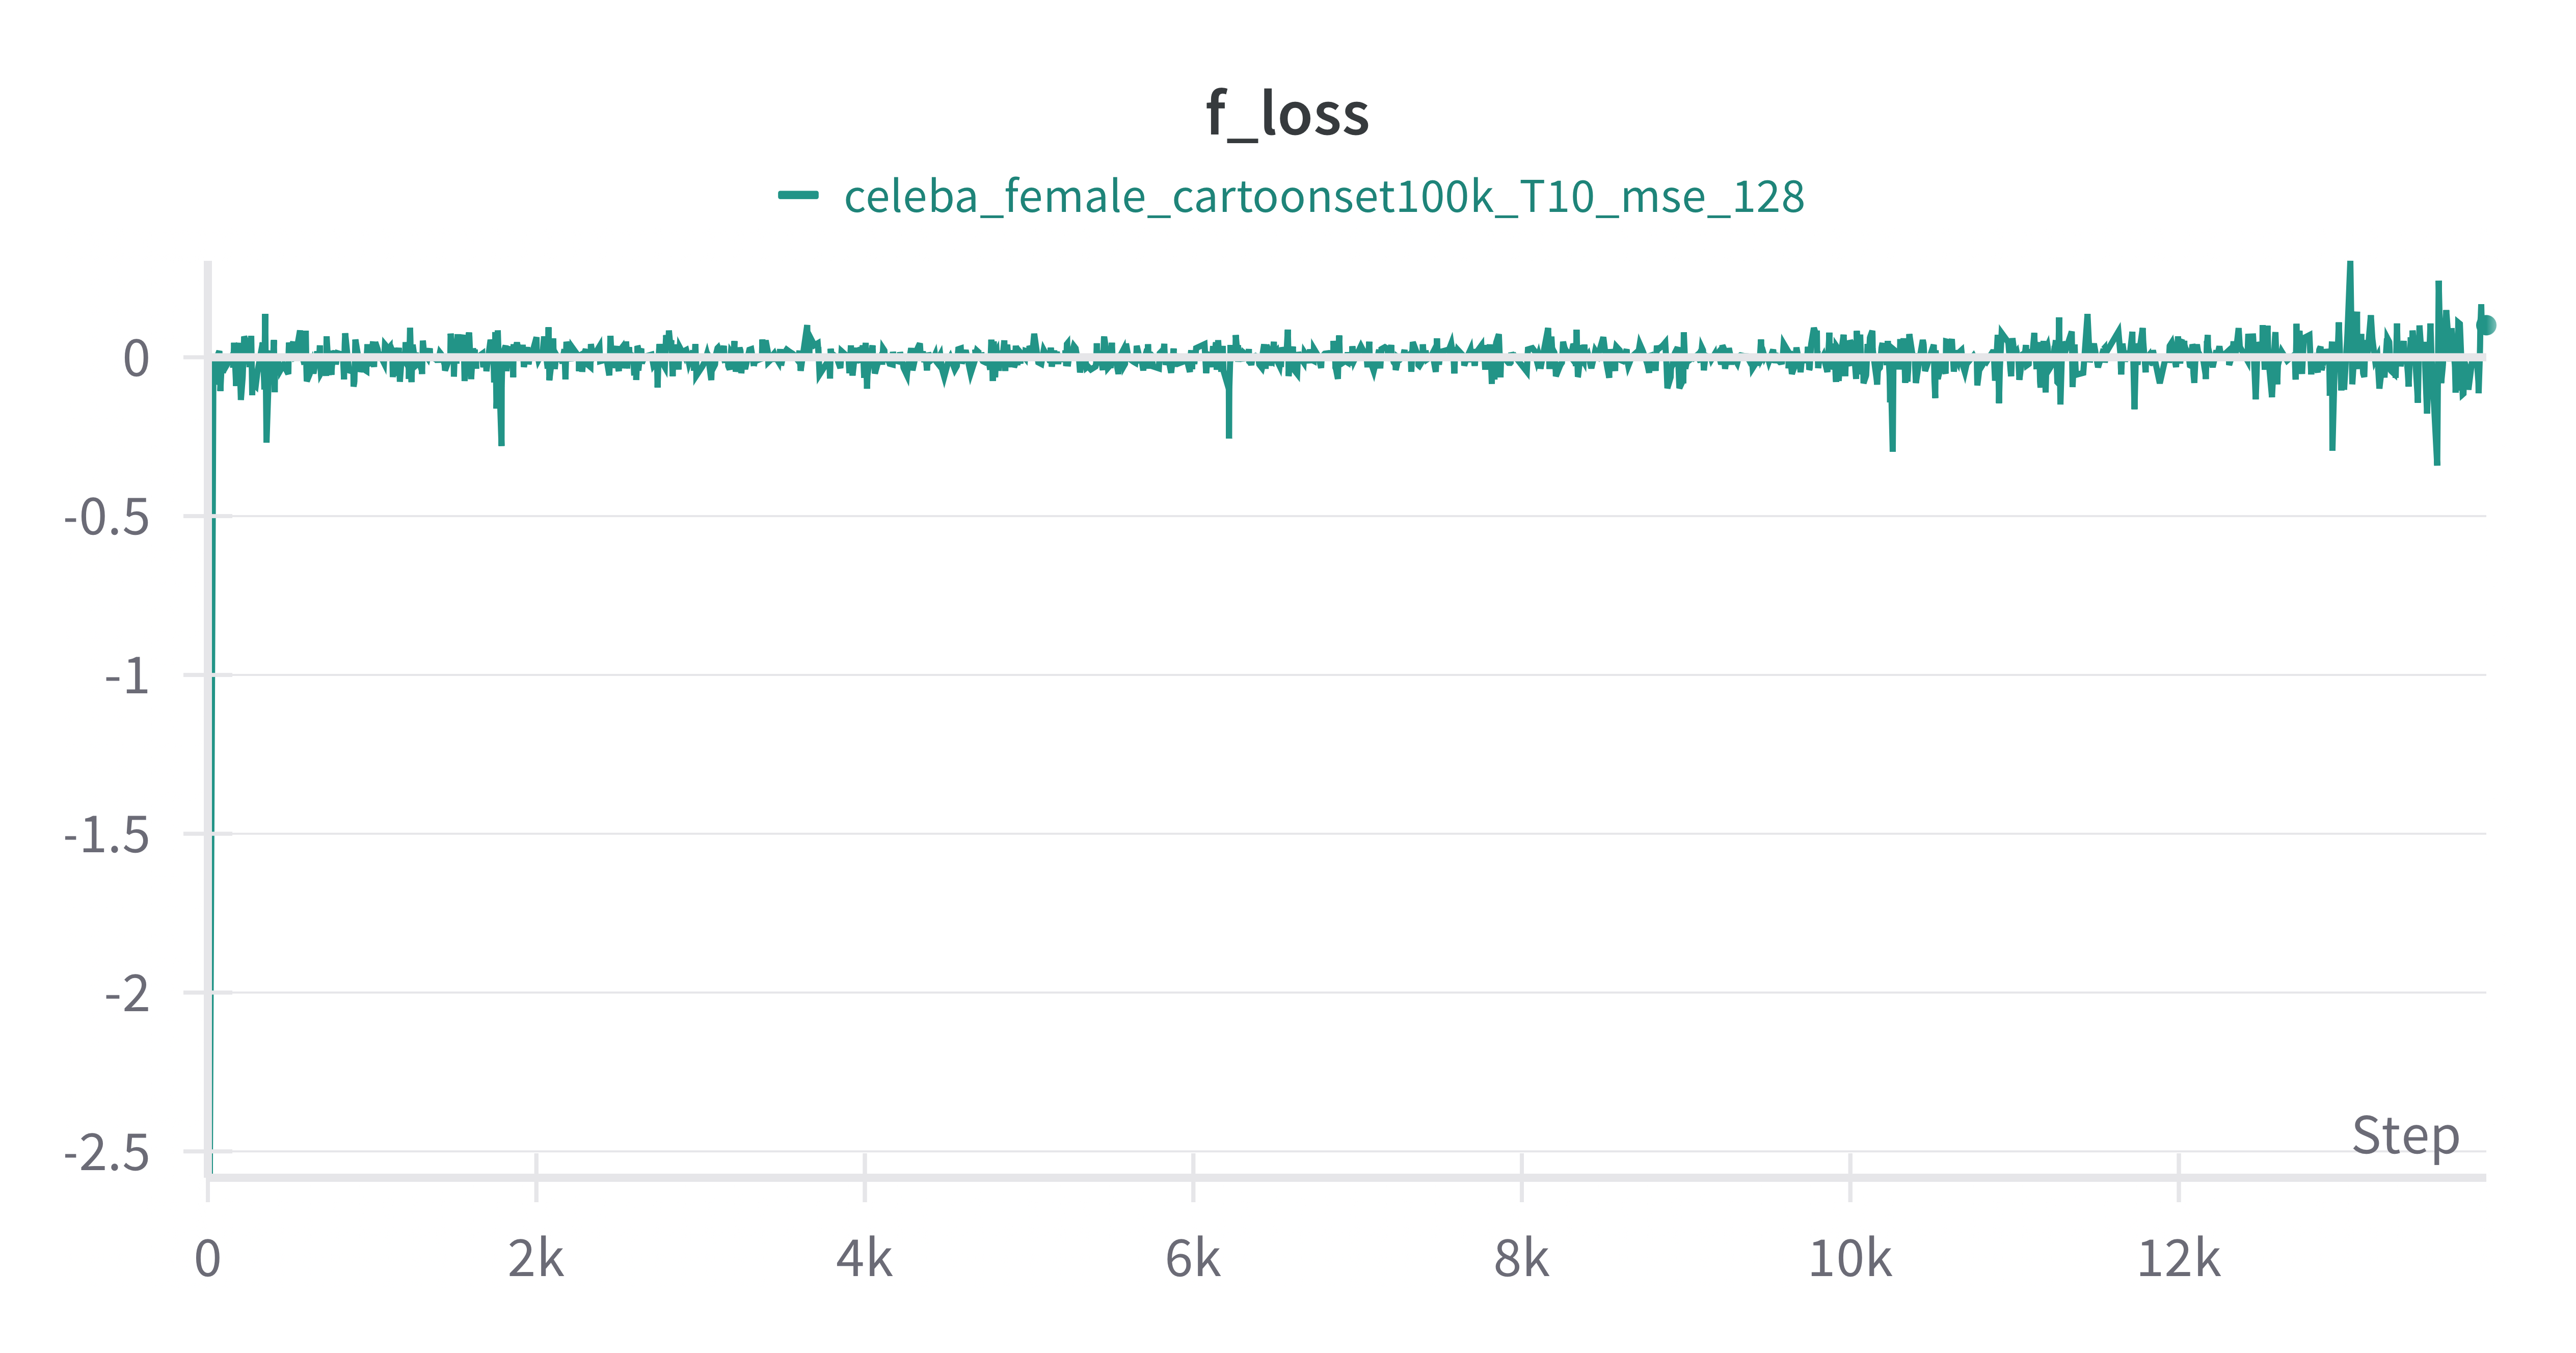
\includegraphics[scale=.05]{figures/loss_real_dataset.png}
    \caption{Loss function}
\end{figure}

\begin{figure}[htp!]
    \centering
    \begin{subfigure}{\textwidth}
        \centering
        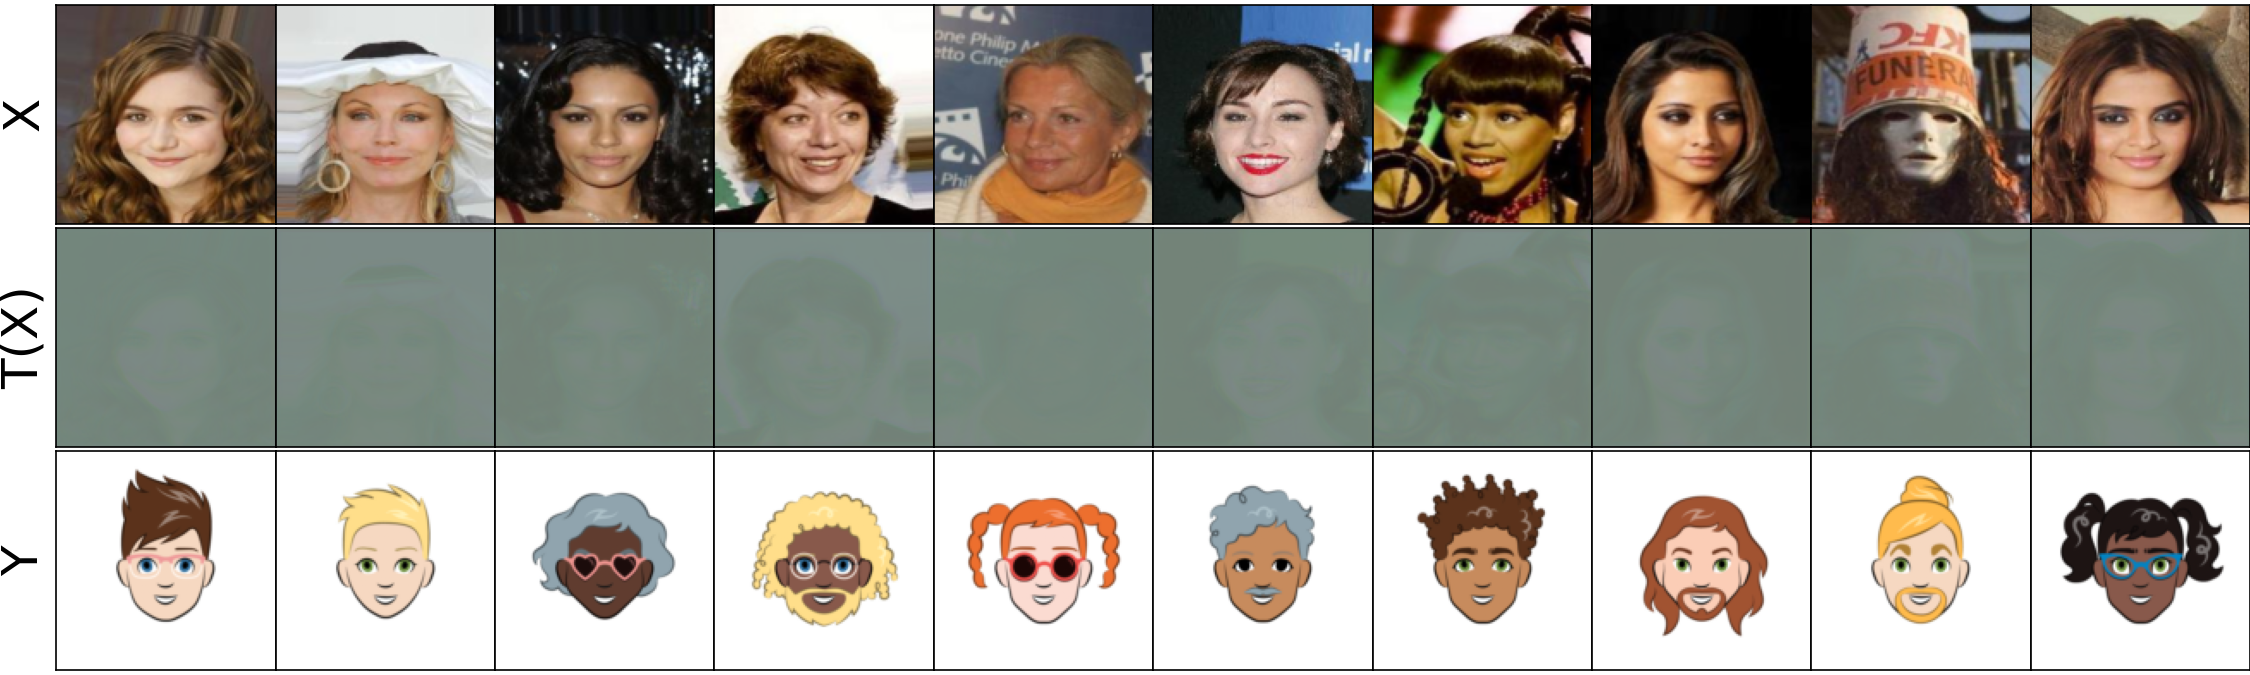
\includegraphics[scale=.15]{figures/media_images_Fixed Images_0_a56284c48d003ecfb6cd.png}
        \caption{Iteration 1}
        \label{fig:test_images_real_iter_1}
    \end{subfigure}%

    \bigskip

    \begin{subfigure}{\textwidth}
        \centering
        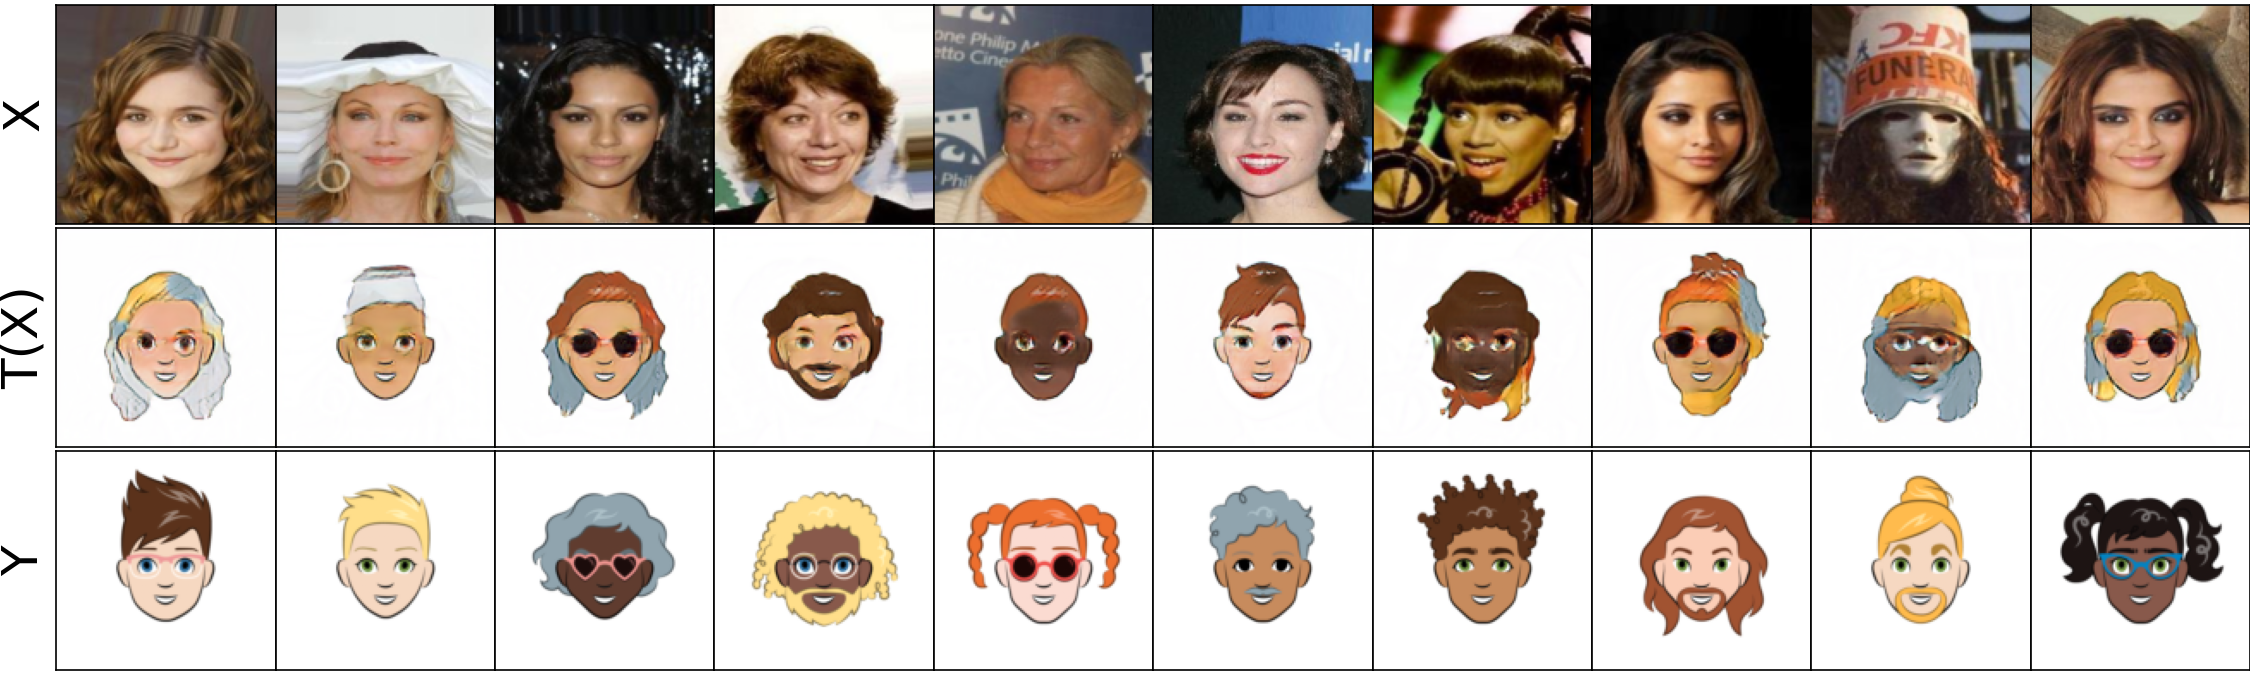
\includegraphics[scale=.15]{figures/media_images_Fixed Images_5000_0043c7527d827202e7ad.png}
        \caption{Iteration 5000}
        \label{fig:test_images_real_iter_med}
    \end{subfigure}%

    \bigskip

    \begin{subfigure}{\textwidth}
        \centering
        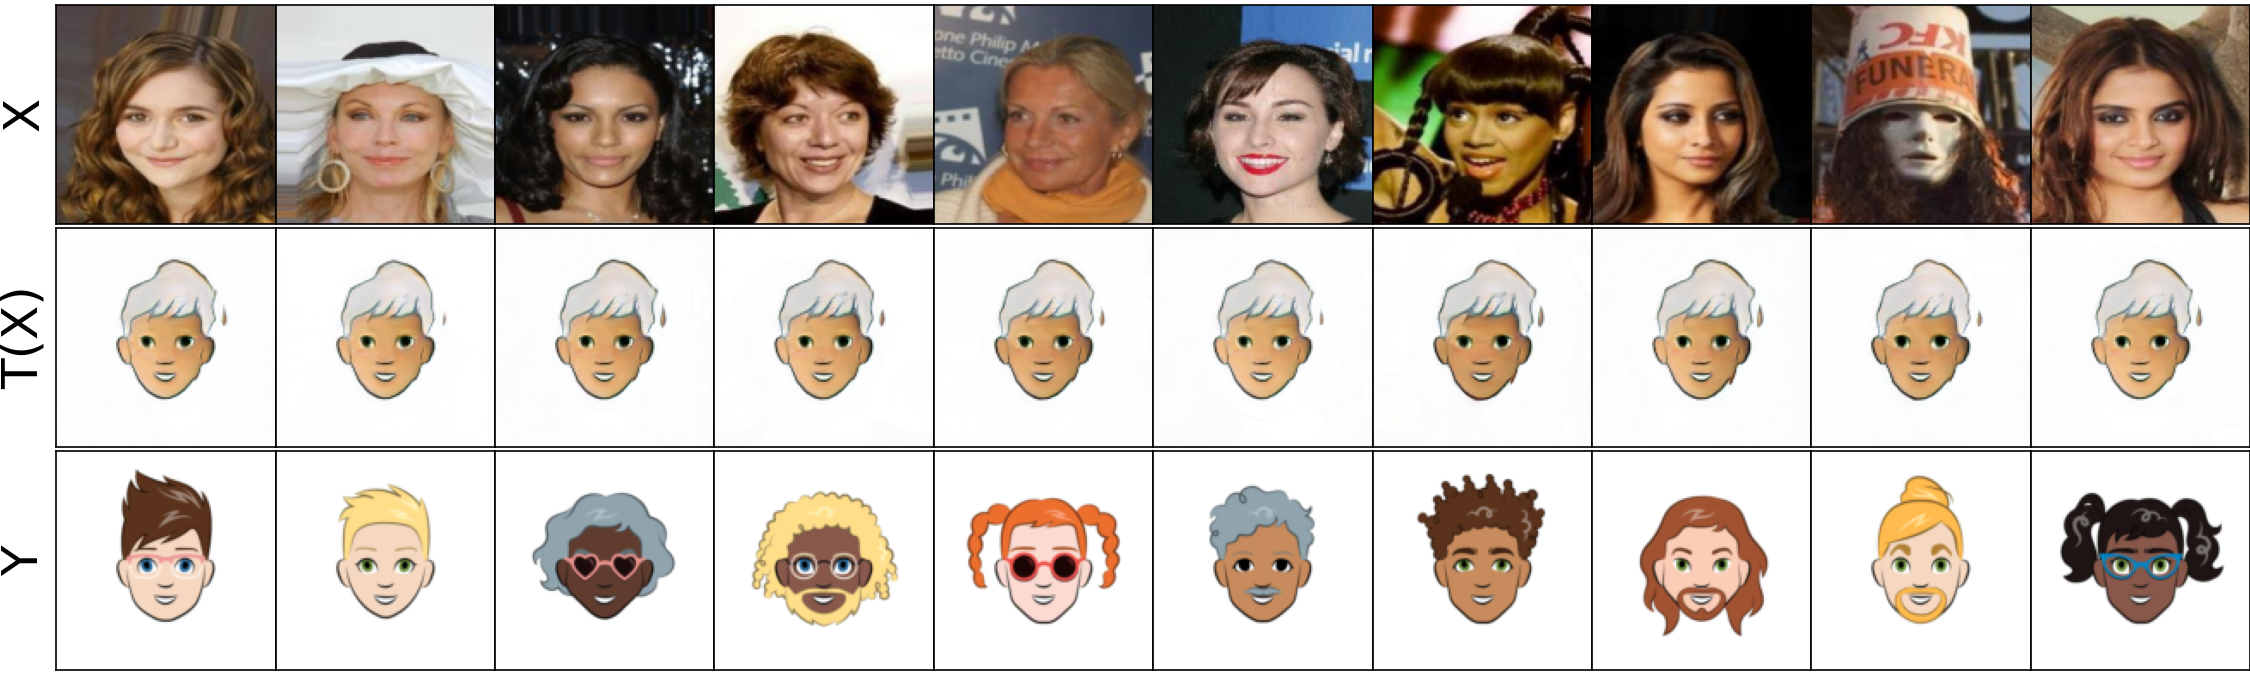
\includegraphics[scale=.15]{figures/media_images_Fixed Images_13800_653d5de40c4ba6a777ca.png}
        \caption{Iteration 13800}
        \label{fig:test_images_real_iter_last}
    \end{subfigure}%
    \caption{Test images}
    \label{fig:test_samples_large_scale}
\end{figure}

Those experiments are quite long in time (about a day for \~15k iterations with the parameters given above) so we restrict ourselves to only train the strong formulation model and the results for a fixed sample of the test set are given in~\ref{fig:test_samples_large_scale}.

\subsubsection{Observations}

Figure~\ref{fig:test_images_real_iter_1} lets us see the model initialisation.

Furthermore, we witnessed realistic mappings of the real faces onto the cartoon avatar distribution around iteration 5000, see~\ref{fig:test_images_real_iter_med}. This is far less than what the authors observed in their experiments, this number was closer to 40k iterations for convergence. However, our images have an empty background so it might be easier in comparison with anime face images which contain a complex surrounding as they are extracted from animes. One can see that the color of the skin and the hair map well. However, the model struggles when there are glasses on the target image. It translates glasses into dark black holes. It's very surprising to see new avatars thanks to those mappings.

At this point, we thought we were far from the end and we decided to continue the training for a night. Unfortunately, few thousands iterations later mode collapses appeared with the same avatar being mapped for a given batch. Surprisingly, the constant predicted face is changing with training without changing the mode collapse.

\section{Conclusion}

In this project, we studied the paper "Neural Optimal Transport" (Korotin, 2023) \cite{korotin-2022} which introduces an algorithm to train a neural network to learn the wrak optimal transport between two distributions. We conducted experiments using synthetic data and a real dataset, and obtained results similar to the ones in the paper. We also observed that the model is quite sensitive to hyperparameters such as the batch size and the number of iterations for the optimization of $T_\theta$. We also observed that the model is prone to mode collapse, which is a common issue in generative modeling. Overall, we found that the algorithm is effective at learning the optimal transport between two distributions, and that it can be used for generative modeling tasks.

\newpage
\bibliography{bibliography}

\newpage
\appendix

\begin{center}
    {\Large \bfseries \scshape Appendix} \\
\end{center}

\section{Figures}

\end{document}
